\documentclass[12pt,a4paper]{article} 
\usepackage{../riemlabm}
\title{Searle's double bar experiment}
\usepackage{fancyhdr}
\lfoot{Regional Institute of Education Mysore}
\lhead{Searle's double bar experiment}
\chead{}
\rhead{Semester 6}
\cfoot{}
\rfoot{Physics}
\pagestyle{fancy}
\begin{document}
	\maketitle
	
	\section{OBJECTIVES}
		To determine the 
			\begin{enumerate}
				\item Young's modulus ($q$) of the material of a wire by flexural oscillations.
				\item Rigidity modulus ($\eta$) by torsional oscillations. 
				\item Poisson's ratio ($\sigma$) for the wire.
			\end{enumerate}
	
	\section{REQUIREMENTS}
		Two metal bars of equal length, breadth and mass, specimen wire, thread, vernier callipers, screw gauge and scale
		
	\section{INTRODUCTION}
		
		The moment of inertia $I$ of a uniform longitudinal bar of length $L$ and mass $M$ about an axis passing through its perpendicular bisector is given by
		
			
			\begin{equation}
				I = \dfrac{M\left(L^2 + b^2\right)}{12}  \label{eq:1}
			\end{equation}
		
		\subsection{Young's Modulus}
			Consider a wire of length $l$ and diameter $d$. Let length $l$ increases by an amount $\Delta l$ when wire is pulled by a longitudinal force $F$. The Young's modulus of the material of a wire is given by, 
			
			\[q = \dfrac{\text{stress}}{\text{strain}}=\dfrac{F/A}{\Delta l/l}\]	
				
			For a uniform bar of length $L$ oscillating with a time period $T_{1}$, the young's modulus can be calculated using the formula
				\begin{equation}
					q=\dfrac{8\pi Il}{T^{2}_{1}r^{4}}
				\end{equation}
				
			where $I$ is the moment of inertia of the uniform bar and $r$ its radius of cross-section.
			
		\subsection{Rigidity Modulus}
			
			The rigidity modulus is given by
				\begin{equation}
				\eta=\dfrac{8\pi Il}{T^{2}_{2}r^{4}}
				\end{equation}
		
		\subsection{Poisson's Ratio}
			The poisson's ratio is given by
			\begin{equation}
				\sigma = \dfrac{q}{2\eta} - 1
			\end{equation}
	\section{PROCEDURE}
		
		\begin{figure}[!htb]
			\centering
			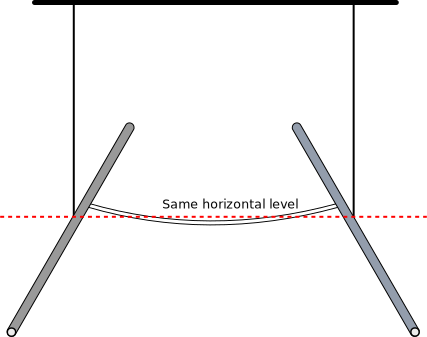
\includegraphics[scale=0.7]{double-bar-diagram.pdf}
			\caption{The experimental setup}
		\end{figure}
		\subsection{To determine the Young's modulus (q)}
		\begin{enumerate}
			\item	The two ends of experimental wire are fixed at the centre of two identical inertia bars.
			
			\item	The two bars are suspended by means of two equal lengths of thread parallel to each other, adjusted such that the two bars are lying in the same plane.
			
			\item	The experimental wire is bent into an arc of a circle. The thread is turned and the system is allowed to execute flexural oscillations in a horizontal plane.
			
			\item	A vertical pointer is fixed on the table to serve as a reference mark for counting the number of oscillations made by one of the inertia bars. Method of difference is also employed to determine the period of oscillations ($T_{1}$) of the system. 
			
			\item	The length $l$ of the experimental wire is measured using a screw gauge; the diameter of the wire is measured at different points along its length, and the mean radius of cross-section $r$ is determined.
			
			\item	The mass $m$ of either of the bars is found. The length $L$ and the mean breadth and thickness of the inertia bar is also measured using slide callipers. 
			
			\item	The moment of inertia $I$ of the bars is calculated about its axis of rotation using the equation  \ref{eq:1}.
		\end{enumerate}
		
		\subsection{To determine the rigidity modulus ($\eta$)}
		
				\begin{figure}[!htb]
					\centering
					\includegraphics[scale=0.6]{flexural.pdf}
					\caption{Flexural oscillations}
				\end{figure}
				
		\begin{enumerate}
			
			\item 	One of the bars is suspended so that it can execute torsional oscillations in a horizontal plane.
			
			\item 	By the method of difference the time period ($T_{2}$).
			
			\item	The length $l$, the radius of cross-section $r$ and moment of inertia $I$ of the experiment wire are determined.
		\end{enumerate}
	\section{OBSERVATIONS}
	
		\subsection{To determine Young's modulus ($q$)}
			
			To determine the time period $T_{1}$,
			\subsubsection{Method 1}
			\begin{center}
				\begin{tabular}{|c|c|c|c|}
				\hline
				\rowcolor{b1!50}Trials&	No. of oscillations&	Time&	Mean period \\
				\rowcolor{b1!50}& &(s) &$t_{1}$ (s) \\ \hline
				1& 10&& \\ \hline
				2& 10&& \\ \hline
				3& 10&& \\ \hline
				4& 10&& \\ \hline
				5& 10&& \\ \hline								
			\end{tabular}
			\end{center}
			\vspace{5pt}
			From the above data, mean $t_{1} = $ \rule{20ex}{0.2pt}
			\subsubsection{Method of difference}
			 \begin{center}
			 	\begin{tabular}{|c|c|c|c|}
			 	\hline
			 	\rowcolor{b1!50}Count&	Time recorded&	Time difference&	Time period \\
			 	\rowcolor{b1!50}of oscillations& &for two oscillations (s) &$t_{2}$ (s) \\ \hline
			 	2& && \\ \hline
			 	4& && \\ \hline
			 	6& && \\ \hline
			 	8& && \\ \hline
			 	10& && \\ \hline					
			 \end{tabular}
				 
				 \vspace{11pt}
				 Mean $T_{1} = \dfrac{t_{1}+t_{2}}{2}= \rule{20ex}{0.2pt}$
			 \end{center}
		\subsection{To determine the rigidity modulus ($\eta$)}
			
			To determine the time period $T_{2}$
			\subsubsection{Method 1}
			\begin{center}
				\begin{tabular}{|c|c|c|c|}
					\hline
					\rowcolor{b1!50}Trials&	No. of oscillations&	Time&	Mean period \\
					\rowcolor{b1!50}& &(s) &$t_{1}$ (s) \\ \hline
					1& 10&& \\ \hline
					2& 10&& \\ \hline
					3& 10&& \\ \hline
					4& 10&& \\ \hline
					5& 10&& \\ \hline								
				\end{tabular}
			\end{center}
			
			\subsubsection{Method of difference}
			\begin{center}
				\begin{tabular}{|c|c|c|c|}
					\hline
					\rowcolor{b1!50}Count&	Time recorded&	Time difference&	Time period \\
					\rowcolor{b1!50}of oscillations& &for two oscillations (s) &$t_{2}$ (s) \\ \hline
					2& && \\ \hline
					4& && \\ \hline
					6& && \\ \hline
					8& && \\ \hline
					10& && \\ \hline					
				\end{tabular}\\
				\vspace{11pt}
				Mean $T_{2} = \dfrac{t_{1}+t_{2}}{2} = \rule{20ex}{0.2pt}$
			\end{center}
			
			
		\subsection{To determine the radius of cross-section of the wire}
		
			Diameter of cross-section $d = \rule{20ex}{0.2pt}$
			\vspace{11pt}\\
			Radius of cross-section $r=\dfrac{d}{2} = \rule{20ex}{0.2pt}$
			\vspace{11pt}\\
			Mass of the bar = \rule{20ex}{0.2pt}
			\vspace{5pt}\\
			Length of the bar = \rule{20ex}{0.2pt}

	\section{CALCULATIONS}
		
		The young's modulus of the material of the wire is calculated using the relation (2). The rigidity modulus is calculated using the relation (3).
		
	\section{RESULT}
		\begin{enumerate}
			\item The Young's modulus ($q$) of the material of the given wire is determined to be \rule{20ex}{0.2pt}
			\item Rigidity modulus ($\eta$) is calculated to be \rule{20ex}{0.2pt}
			\item Poisson's ratio ($\sigma$) for the wire is calculated to be \rule{20ex}{0.2pt}
		\end{enumerate}
		
	
\end{document}
